\documentclass{beamer}
\usepackage{geometry}
\usepackage[english]{babel}
\usepackage[utf8]{inputenc}
\usepackage{amsmath}
\usepackage{amsfonts}
\usepackage{amssymb}
\usepackage{tikz}
\usepackage{graphicx}
\usepackage{venndiagram}

%\usepackage{pgfplots}
%\pgfplotsset{width=10cm,compat=1.9}
%\usepackage{pgfplotstable}

\setlength{\headheight}{26pt}%doesn't seem to fix warning

\usepackage{fancyhdr}
\pagestyle{fancy}
\fancyhf{}

%\rhead{\small{21 May 2018}}
\lhead{\small{BECA / Dr. Huson / 12.1 IB Math - Unit 5 Integration}}

%\vspace{1cm}

\renewcommand{\headrulewidth}{0pt}


\title{12.1 IB Math - Unit 5: Integration}
\subtitle{Bronx Early College Academy}
\author{Christopher J. Huson PhD}
\date{4 January 2019}

\begin{document}

\frame{\titlepage}

\section[Outline]{}
\frame{\tableofcontents}

\section{5.1 Drui: Antiderivatives. Friday 4 January}
  \frame
  {
  \frametitle{GQ: How do we find the antiderivative of a function?}
  \framesubtitle{CCSS: F.IF.B.6 Calculate \& interpret rate of change \hfill \alert{5.1 Friday 4 January}}

  \begin{block}{Do Now. Find $\frac{\mathrm{d}y}{\mathrm{d}x}$}
  \begin{enumerate}
      \item Given $y=x^3+x^2+17$.
      \item Given $y=\frac{1}{4}x^4+\frac{1}{2}x^2+9-\frac{1}{x}$.
      \item If $\displaystyle \frac{\mathrm{d}y}{\mathrm{d}x}=3x^2+x$, find $y$.
      \item Skills check \#1 p. 290
  \end{enumerate}
  \end{block}
  Problem sets from January 2,3; Sigma notation, p 290 \\*[5pt]
  Lesson: Antiderivatives pp. 291-2\\*[5pt]
  Exam review \\*[5pt]
  Homework: Exercises 9A p. 293; test corrections due Monday
}

\section{5.2 Drui: Indefinite Integral. Monday 7 January}
  \frame
  {
  \frametitle{GQ: How do we find the indefinite integral of a function?}
  \framesubtitle{CCSS: F.IF.B.6 Calculate \& interpret rate of change \hfill \alert{5.2 Monday 7 January}}

  \begin{block}{Do Now. Find the antiderivative, $F(x)$, of each function, $f(x)$, such that $F'(x)=f(x)$}
  \begin{enumerate}
      \item $f(x)=4x^3+3x^2+1$.
      \item $f(x)=x^4+x^2+5$.
      \item $f(x)= \sqrt{x}$
  \end{enumerate}
  \end{block}
  Test corrections due, review. (take home test tomorrow)\\*[5pt]
  Lesson: Indefinite integral pp. 293-4\\*[5pt]
  Homework: Exercises 9B p. 294
}

\section{5.3 Drui: Deltamath Integration Tuesday 8 January}
  \frame
  {
    \frametitle{GQ: How do we integrate functions?}
    \framesubtitle{CCSS: F.IF.B.6 Calculate \& interpret rate of change \hfill \alert{5.3  Tuesday 8 January}}

    \begin{block}{Do Now. Handout-test review}
      %\begin{enumerate}

      %\end{enumerate}
    \end{block}
    Deltamath Integration practice (taking antiderivatives)\\*[5pt]
    Homework: Deltamath project through Thursday
  }

\section{5.4 Drui: Boundary conditions. Wednesday 9 January}
  \frame
  {
  \frametitle{GQ: How do we apply boundary conditions to an integral?}
  \framesubtitle{CCSS: F.IF.B.6 Calculate \& interpret rate of change \hfill \alert{5.4 Wednesday 9 January}}

  \begin{block}{Do Now. Find each indefinite integral.}
  \begin{enumerate}
      \item $\int (3x^2+2x+1) \,\mathrm{d}x$.
      \item $\int (x^4+6x^2+1) \,\mathrm{d}x$.
      \item $\int \sqrt{x} \,\mathrm{d}x$.
      \item $\displaystyle \int \frac{\pi}{4} \sqrt[3]{x^2} \,\mathrm{d}x$
      \item $\int x^{-1} \,\mathrm{d}x$
  \end{enumerate}
  \end{block}
  Lesson: Finding the constant $C$ given boundary conditions. pp. 295-6\\*[5pt]
  Homework: Exercises 9C p. 296-7
}

\section{5.5 Drui: Deltamath Integration Thursday 10 January}
  \frame
  {
  \frametitle{GQ: How do we integrate functions?}
  \framesubtitle{CCSS: F.IF.B.6 Calculate \& interpret rate of change \hfill \alert{5.5  Thursday 10 January}}

  \begin{block}{Do Now. Handout-test review}
    %\begin{enumerate}

    %\end{enumerate}
  \end{block}
  Deltamath Integration practice (taking antiderivatives)\\*[5pt]
  Homework: Complete Deltamath calculus project
}

\section{5.6 Drui: Compositions of linear functions. Friday 11 January}
  \frame
  {
  \frametitle{GQ: How do we integrate compositions of linear functions?}
  \framesubtitle{CCSS: F.IF.B.6 Calculate \& interpret rate of change \hfill \alert{5.6 Friday 11 January}}

  \begin{block}{Do Now. Derivatives and antiderivatives. (Use the chain rule)}
  \begin{enumerate}
    \item $f(x)=e^{3x}$. Find $f'(x)$.
    \item $f(x)= \ln (5x+3)$. Find $f'(x)$.
    \item $f(x)= (2x-5)^3$. Find $f'(x)$.

    \item Find $\int 4(x^2+x+1) \,\mathrm{d}x$.
    \item $y'=2x^3-1$ and $y=3$ when $x=1$. Find $y$ in terms of $x$.
    \item Given $f'(x)=\sqrt[3]{x}$ and $f(0)=1$, find $f(x)$.
  \end{enumerate}
  \end{block}
  Lesson: Antiderivatives of form $\int f(ax+b) \,\mathrm{d}x$. pp. 297-9\\*[5pt]
  Homework: Exercises 9D, 9E (odds) p. 298, 300
}

\section{5.7 Drui: Compositions of linear functions. Monday 14 January}
  \frame
  {
  \frametitle{GQ: How do we integrate compositions of linear functions?}
  \framesubtitle{CCSS: F.IF.B.6 Calculate \& interpret rate of change \hfill \alert{5.7 Monday 14 January}}

  \begin{block}{Do Now. Derivatives and antiderivatives. (Use the chain rule)}
  \begin{enumerate}
    \item $f(x)=e^{2x-3}$. Find $f'(x)$.
    \item $f(x)= \ln (4x)$. Find $f'(x)$.
    \item $f(x)= (3x+2)^4$. Find $f'(x)$.

    \item Find $\int (5x^3+x^2+1) \,\mathrm{d}x$.
    \item $y'=2x^2-1$ and $y=3$ when $x=3$. Find $y$ in terms of $x$.
    \item Given $f'(x)=\sqrt[3]{x^2}$ and $f(1)=1$, find $f(x)$.
  \end{enumerate}
  \end{block}
  Lesson: Antiderivatives of form $\int f(ax+b) \,\mathrm{d}x$. pp. 297-9\\*[5pt]
  Homework: Exercises 9D, 9E (evens) p. 298, 300
}

\section{5.8 Drui: Deltamath Integration Tuesday 15 January}
  \frame
  {
  \frametitle{GQ: How do we integrate functions?}
  \framesubtitle{CCSS: F.IF.B.6 Calculate \& interpret rate of change \hfill \alert{5.8  Tuesday 15 January}}

  \begin{block}{Do Now. Straight to DeltaMath}
    %\begin{enumerate}

    %\end{enumerate}
  \end{block}
  Deltamath Integration practice (taking antiderivatives)\\*[5pt]
  Homework: Complete Deltamath
}

\section{5.9 Drui: Integration - position problems. Wednesday 16 January}
  \frame
  {
  \frametitle{GQ: How do we use integration to solve for position?}
  \framesubtitle{CCSS: F.IF.B.6 Calculate \& interpret rate of change \hfill \alert{5.9 Wednesday 16 January}}

  \begin{block}{Do Now. Derivatives and antiderivatives.}
  \begin{enumerate}
    \item $f(x)=\sin x$. Find $f'(x)$.
    \item Find $\int \sin x \,\mathrm{d}x$.

    \item $s(t)= 4.9 t^2$. Find $v(t)=s'(t)$ and $a(t)=s''(t)$.\\
    What might these functions represent?

    \item Given $v(t)=\cos t$, find $s(t)=\int v(t) \,\mathrm{d}t$. Assume $s(0)=0$.

  \end{enumerate}
  \end{block}
  Lesson: Position problems (handout)\\*[5pt]
  Homework: Calculus problem set
}

\section{5.10 Drui: Definite integrals and area. Thursday 17 January}
  \frame
  {
    \frametitle{GQ: How do we calculate area with integration?}
    \framesubtitle{CCSS: F.IF.B.6 Calculate \& interpret rate of change \hfill \alert{5.10 Thursday 17 January}}

    \begin{block}{Do Now}
    \begin{enumerate}
        \item Find $\int{(4x^3-3x+1)}\mathrm{d}x$.
        \item Find $\int e^{5x}\mathrm{d}x$.
        \item Find $\displaystyle \int \frac{1}{3x+1} \mathrm{d}x$.
    \end{enumerate}
    Homework review \#1, 5, 6 p. 302
    \end{block}
    Lesson: Reimann sums and the definite integral\\*[5pt]
    Task: Example 8, page 304\\*[5pt]
    Assessment: Calculator integration \\*[5pt]
    Homework: Exercises 9H evens p. 308
  }

\section{5.11 Definite integrals and area. Friday 18 January}
  \frame
  {
    \frametitle{GQ: How do we calculate area with definite integrals?}
    \framesubtitle{CCSS: F.IF.B.6 Calculate \& interpret rate of change \hfill \alert{5.11 Friday 18 January}}

    \begin{block}{Do Now}
    \begin{enumerate}
        \item Use a calculator to find $\displaystyle \int_0^{\frac{\pi}{2}}{\cos x}\ \mathrm{d}x$
        \item Differentiate $y=\sqrt{3x^3-x}$
        \item Find $\int{(6x^2-2x-5)}\mathrm{d}x$.
        \item Differentiate $y={(3x^2-5x)^5}$
        %\item Find $\int 5(x^2+1)^4(2x)\mathrm{d}x$.
        \item Find $\displaystyle \int \frac{3}{x}\ \mathrm{d}x$.
    \end{enumerate}
    \end{block}
    Lesson: Properties of definite integrals p. 307\\
    The fundamental theorem of calculus p. 309\\*[5pt]
    Homework: Have a nice break!
  }

\section{5.12 Deltamath: definite integrals and area. Tuesday 29 January}
  \frame
  {
    \frametitle{GQ: How do we calculate area with definite integrals?}
    \framesubtitle{CCSS: F.IF.B.6 Calculate \& interpret rate of change \hfill \alert{5.12 Tuesday 29 January}}

    \begin{block}{Do Now: 6-1 Calculus Tangent lines spiral review handout}
    \begin{enumerate}
        \item Select and solve one of the problems: mild, medium, or spicy. (early finishers, do another)
        \item As a class, check work
        \item Record result in personal tracker
    \end{enumerate}
    \end{block}
    Lesson: Definite integrals\\%*[5pt]
    Task: Deltamath practice\\%*[5pt]
    Homework: Exercises 9I p. 310-1
  }

\section{5.13 Integration by substitution. Wednesday 30 January}
  \frame
  {
    \frametitle{GQ: How do we anti-differentiate using the chain rule?}
    \framesubtitle{CCSS: F.IF.B.6 Calculate \& interpret rate of change \hfill \alert{5.13 Wednesday 30 January}}

    \begin{block}{Do Now}
    \begin{enumerate}
        \item Differentiate $y=\sqrt[3]{5x^2-2x}$
        \item Find $\int{(6x-2)^4(6)} \ \mathrm{d}x$.
        \item Differentiate $y={(3x^2-5x)(\ln x)}$
        \item Use a calculator to find $\displaystyle \int_{-1}^{1}{\frac{1}{x+2}}\ \mathrm{d}x$
        \item Find $\displaystyle \int_1^2 \frac{3}{x^2}\ \mathrm{d}x$. (check your result with a calculator)
    \end{enumerate}
    \end{block}
    Lesson: The substitution method of integration p. 300\\%*[5pt]
    Task: Practice Examples 7 p. 300\\%*[5pt]
    Homework: Exercises 9J p. 312-13
  }

\section{Cold-day 6-1 P1 Tangents A spiral review. Thursday 31 January}
  \frame
  {
    \frametitle{GQ: How do we find the tangent of a curve?}
    \framesubtitle{CCSS: F.IF.B.6 Calculate \& interpret rate of change \hfill \alert{Cold-day, Thursday 31  January}}

    \begin{block}{Do Now}
    \begin{enumerate}
        \item 6-1 P1 Tangents A spiral review
    \end{enumerate}
    \end{block}
    Homework: 6-1 P1 Tangents B spiral review
  }

\section{5.14 Deltamath: Area between two curves. Friday 1 February}
  \frame
  {
    \frametitle{GQ: How do we calculate the area between two curves?}
    \framesubtitle{CCSS: F.IF.B.6 Calculate \& interpret rate of change \hfill \alert{5.14 Friday 1 February}}

    \begin{block}{Do Now: 6-1 Calculus Tangents spiral review handout \\ Early finishers - Take the derivative of each function}
      \begin{enumerate}
      \item $f(x)=\sin{x^3}$
      \item $g(x)=\sqrt{x^4+2}$
      \item $h(x)=\ln{(x^2+1)}$
      \end{enumerate}
   \end{block}
    Lesson: The area between two functions p. 313\\%*[5pt]
    %Task: Practice Examples 11, 12 p. 310-1\\%*[5pt]
    Assessment: Example \#13 p. 314 \\%*[5pt]
    Homework: Exercises 9K p. 316
  }

\section{5.15 Area between two curves. Monday 4 February}
  \frame
  {
    \frametitle{GQ: How do we calculate the area between two curves?}
    \framesubtitle{CCSS: F.IF.B.6 Calculate \& interpret rate of change \hfill \alert{5.15 Monday 4 February}}

    \begin{block}{Do Now: Integration practice}
    \begin{enumerate}
      \item $\int (x^2+2x+7) \,\mathrm{d}x$.
      \item $\int (\sin x + \frac{1}{x} - \sqrt{x}) \,\mathrm{d}x$.
      \item $\int e^{3x-4} \,\mathrm{d}x$.
      \item $\displaystyle \int \frac{3x^2+5}{(x^3+5x)^3} \,\mathrm{d}x$
      \item $\displaystyle \int_0^2 2 \sqrt{2x-x^2} \,\mathrm{d}x$ (use a calculator)
    \end{enumerate}
    \end{block}
    Homework review \#9K p. 316\\
    Lesson: Determining definite integrals' boundaries p. 317\\%*[5pt]
    Assessment: Example \#14 p. 317 (\alert{test Thursday})\\%*[5pt]
    Homework: Pre-test; 6-2 P1 Differentiation spiral review
  }

\section{5.16 Test review. Wednesday 6 February}
  \frame
  {
    \frametitle{GQ: How do we calculate the area between two curves?}
    \framesubtitle{CCSS: F.IF.B.6 Calculate \& interpret the rate of change \hfill \alert{5.16 Wednesday 6 February}}

    \begin{block}{Do Now: Integration practice}
    \begin{enumerate}
      \item $\displaystyle \int_0^{\frac{\pi}{2}} \sin x \,\mathrm{d}x$ (Do this without a calculator. Sketch the unit circle.)
    \end{enumerate}
    \end{block}
    6-2 P1-A Differentiation spiral review\\
    Lesson: Pretest review (\alert{test tomorrow})\\%*[5pt]
    Homework: Study for exam.\\
    6-2 P1-B Differentiation spiral review (Friday)
  }

\section{5.17 Unit test: Integration. Thursday 7 February}
\frame
{
  \frametitle{GQ: How do we calculate the area between two curves?}
  \framesubtitle{CCSS: F.IF.B.6 Calculate \& interpret rate of change\hfill \alert{5.17 Thursday 7 February}}
  \alert{Unit test:} Antidifferentiation, definite integrals, finding areas\\%*[5pt]
  Homework: Exercises \#9L 317
}

\section{5.18 Calculus overview review. Friday 8 February}
  \frame
  {
    \frametitle{GQ: How do we calculate the area between two curves?}
    \framesubtitle{CCSS: F.IF.B.6 Calculate \& interpret rate of change \hfill \alert{5.18 Friday 8 February}}

    \begin{block}{Do Now: Integration practice}
    \begin{enumerate}
      \item $\displaystyle \int_0^{\frac{\pi}{2}} \sin x \,\mathrm{d}x$
    \end{enumerate}
    \end{block}
    Homework review \#9L p. 317\\
    6-2 P1-B Differentiation spiral review\\
    Lesson: Differentiation review, concavity\\%*[5pt]
    Homework: Integration practice; 6-2 P1-C Differentiation spiral review
  }

\section{5.19 Volumes of rotation. Monday 11 February}
  \frame
  {
    \frametitle{GQ: How do we calculate a volume of rotation?}
    \framesubtitle{CCSS: F.IF.B.6 Calculate \& interpret rate of change \hfill \alert{5.15 Monday 11 February}}

    \begin{block}{Do Now: Sketch the functions $f(x)=10x+x^2-3x^3$ and $g(x)=x^2-2x$}
    \begin{enumerate}
        \item What are their intersections? (i.e. $f(x)=g(x)$)
        \item What is the definite integral representing the area between the curves?
        \item Using a calculator, what is the size of the area? (this may not be a trivial question)
    \end{enumerate}
    \end{block}
    Lesson: Integrating circle areas, modeling a solid p. 318\\%*[5pt]
    %Task: Practice Examples 11, 12 p. 310-1\\%*[5pt]
    Assessment: Example \#15 p. 319 \\%*[5pt]
    Homework: Exercises 9L \& 9M p. 317, 319
  }

  \frame
  {
    \frametitle{The volume of a function rotated around the $x$-axis}
    \framesubtitle{Differentiate over $x$, but use the area of a disk defined by $A=\pi r^2$}
  \href{https://www.youtube.com/watch?v=i4L5XoUBD_Q}{video}\\
  \begin{figure}[!ht]
      \centering
      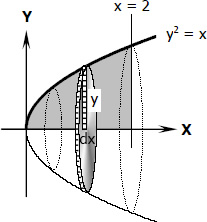
\includegraphics[width=0.5\textwidth]{0413CW-paraboloid.jpg}
  \end{figure}
  \small{Credit: MATHalino.com - Pinoy Math Community Romel Verterra}
  }

\section{5.20 Deltamath volumes of rotation. Tuesday 12 February}


\section{5.21 Volumes of rotation. Wednesday 13 February}
  \frame
  {
    \frametitle{GQ: How do we calculate a volume of rotation?}
    \framesubtitle{CCSS: F.IF.B.6 Calculate \& interpret rate of change \hfill \alert{5.21 Wednesday 13 February}}

    \begin{block}{Do Now: Volumes of rotation}
    \begin{enumerate}
        \item Medium: $f(x)=-x^2+4$.
        \begin{enumerate}
            \item What is the range of $f$? The roots?
            \item Find $f'(x)$.
            \item Find the volume generated when the curve of $f$ for $-2 \leq x \leq 2$ is revolved through $2\pi$ about the $x$-axis.
        \end{enumerate}
        \item Spicy: $g(x)= \sin^3x$.
        \begin{enumerate}
            \item What is the range of $g$?
            \item Find $g'(x)$.
            \item Find the volume generated when the curve of $g$ for $0 \leq x \leq \frac{\pi}{2}$ is revolved through $2\pi$ about the $x$-axis.
        \end{enumerate}
    \end{enumerate}
    \end{block}
    Lesson: Kinematics p. 321\\
    Homework: Textbook exercises (9N p. 320) 9O p. 324-5 \alert{test corrections due Friday (before field trip)}
  }

\section{5.22 Volumes of rotation. Thursday 14 February}
  \frame
  {
    \frametitle{GQ: How do we calculate a volume of rotation?}
    \framesubtitle{CCSS: F.IF.B.6 Calculate \& interpret rate of change \hfill \alert{5.22 Thursday 14 February}}

    \begin{block}{Do Now: Volumes review}
    \begin{enumerate}
        \item Volumes review
    \end{enumerate}
    \end{block}
    Lesson: Integrating circle areas, modeling a solid p. 318\\*[5pt]
    Homework: Problem set \alert{test corrections due tomorrow}
  }

\section{Kinematics (preview)}
  \frame
  {
    \frametitle{GQ: How do we calculate displacement from velocity?}
    \framesubtitle{CCSS: F.IF.B.6 Calculate \& interpret the rate of change of a function \qquad \alert{12.1}}

    \begin{block}{Do Now: Do the calculations below and read the handout}
    \begin{enumerate}
        \item Lance Armstrong’s average speed in his six Tour de France victories from 1999-2004 was about 24 miles per hour. Assuming that he pedals at his average speed and takes no breaks, how long would it take him to ride 38 miles to the top of a 10,000 ft. volcano?
        \item People who are not Lance Armstrong can travel at about 12 miles per hour on a bike. At that speed, how long would it take to reach the top of the volcano?
    \end{enumerate}
    \end{block}
    Lesson: Integrating velocity over time, displacement p. 321\\%*[5pt]
    %Task: Practice Examples 11, 12 p. 310-1\\%*[5pt]
    Assessment: Example \#18 p. 323 \\%*[5pt]
    Homework: Exercises 9N \& 9O p. 320, 324
  }

\section{Kinematics (preview)}
  \frame
  {
    \frametitle{GQ: How do we calculate displacement from velocity?}
    \framesubtitle{CCSS: F.IF.B.6 Calculate \& interpret the rate of change of a function \qquad \alert{12.1}}

    \begin{block}{Do Now: continued, 38 mile ride in 10 hours}
    \begin{enumerate}
        \item Using the velocity vs time graph from yesterday, integrate to show that the areas representing the distance covered by the three riders are equal ($v \times t = d$).
        \item Show that a rider accelerating according to $v(t)= \frac{76}{100}t$ also arrives at $(10,38)$.
    \end{enumerate}
    \end{block}
    Lesson: Integrating velocity over time, displacement p. 321\\%*[5pt]
    Task: Review 9F, 9M, probability\\%*[5pt]
    Assessment: Example \#18 p. 323 (take home test Thursday)\\%*[5pt]
    Homework: Exercises 9P p. 326, any remaining problem sets
  }

\section{5.23 Integration review. Monday 25 February}
  \frame
  {
    \frametitle{GQ: How do we calculate a volume of rotation?}
    \framesubtitle{CCSS: F.IF.B.6 Calculate \& interpret rate of change \hfill \alert{5.23 Monday 25 February}}

    \begin{block}{Do Now: Integration practice review}
    \begin{enumerate}
        \item Review Exercises \#1a, 1b, 1c, \#2a p.327
    \end{enumerate}
    \end{block}
    Lesson: Gabriel's horn p. 331\\
    Practice: medium complete \#1,2 p. 327; spicy 3-7 p. 327\\*[5pt]
    Homework: Complete exam-style problems pp. 327-8
  }

  \section{5.24 Deltamath integration review. Tuesday 26 February}
  \frame
  {
    \frametitle{GQ: How do we use integration to find the area under a function curve or a volume of rotation?}
    \framesubtitle{CCSS: F.IF.B.6 Calculate \& interpret rate of change \hfill \alert{5.24 Tuesday 26 February}}

      \begin{block}{Do Now: Integration practice review}
      \begin{enumerate}
          \item \emph{Medium} - integrate the area under a function
          \item \emph{Spicy} - integrate a volume of rotation
      \end{enumerate}
      \end{block}
    Homework problem set review\\
    Lesson: Deltamath integration and differentiation review\\
    Assessment: \alert{exam Friday}\\*[5pt]
    Homework: Complete Deltamath problem set
  }

\section{Ice skating. Wednesday 27 February}

\section{5.25 Test review. Thursday 28 February}
  \frame
  {
    \frametitle{GQ: How do we use integration?}
    \framesubtitle{CCSS: F.IF.B.6 Calculate \& interpret the rate of change \hfill \alert{5.25 Thursday 28 February}}

    \begin{block}{Do Now: Integration practice}
    \begin{enumerate}
      \item $\displaystyle \int_0^{\frac{\pi}{2}} \cos x \,\mathrm{d}x$ (Do this without a calculator. Sketch the unit circle.)
    \end{enumerate}
    \end{block}
    %6-2 P1-A Differentiation spiral review\\
    Lesson: Pretest review (\alert{test tomorrow})\\%*[5pt]
    Homework: Study for exam.\\
  }

\section{5.26 Unit test: Integration. Friday 1 March}
\frame
{
  \frametitle{GQ: How do we use integration?}
  \framesubtitle{CCSS: F.IF.B.6 Calculate \& interpret rate of change\hfill \alert{5.26 Friday 1 March}}

  \alert{Unit test:} Antidifferentiation, definite integrals, volumes of rotation\\*[5pt]
  Homework: Problem set handout
}

\end{document}
